\begin{block}{Project Features}
    \begin{itemize}
        \item Retrieve and evaluate source code from source code managers
            such as Git and Subversion
        \item Source code analysis scheduling
        \item Use of multiple metric configurations for multiple
            projects
        \item Visualization of historical results via charts
        \item Public results that are accessible by the community
        \item Extensible architecture to include new metric collectors
            Currently, the following collectors are available:
            \begin{itemize}
							\item Analizo (Java, C and C++)
							\item metric\_fu (Ruby)
							\item Radon (Python)
							\item CodeClimatePHPMD (PHP)
            \end{itemize}
    \end{itemize}
\end{block}

\begin{block}{Project: Metric evaluation results}
    \begin{figure}
        \begin{center}
            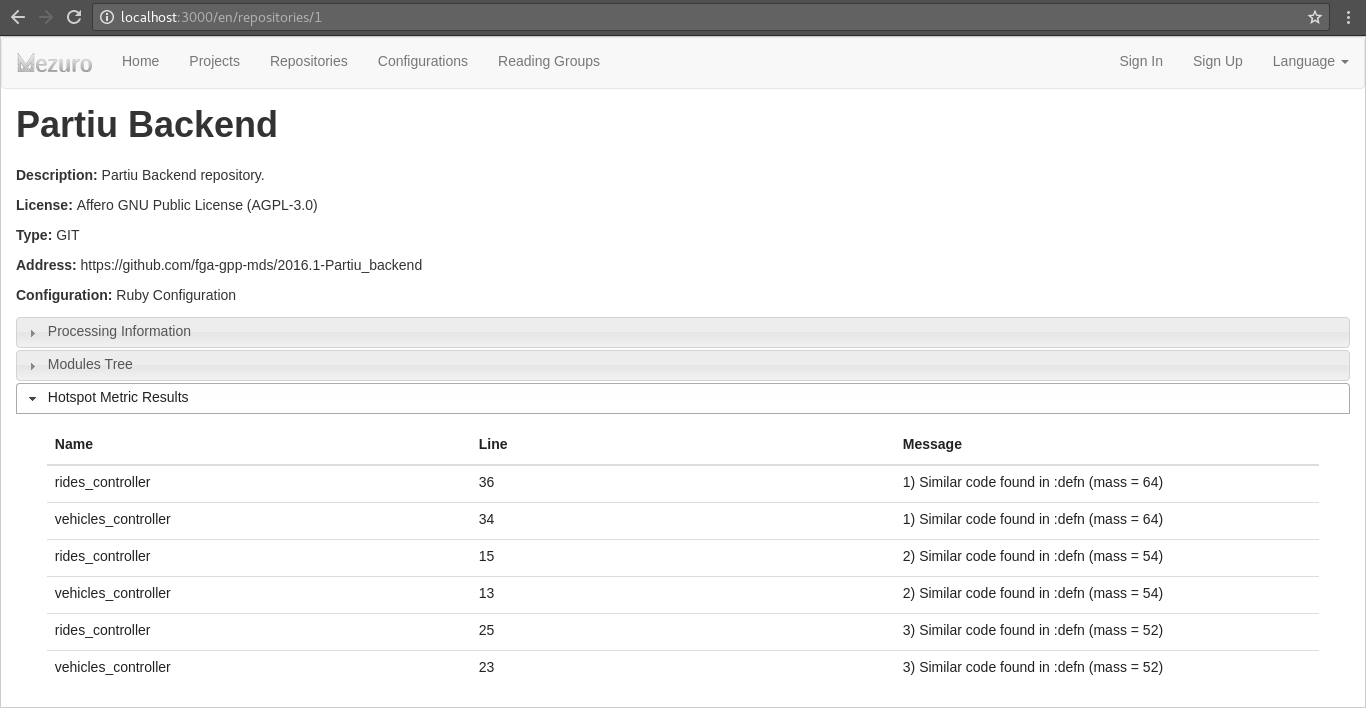
\includegraphics[width=\textwidth]{figures/MetricProcessing.png}
                \label{fig:feature1}
        \end{center}
    \end{figure}
\end{block}

\begin{block}{Metric Configurations Features}
    \begin{itemize}
        \item Metric configurations are responsible for allowing
            definitions and spread of metrics configurations, being
            one of Mezuro stand out factors among the others platforms
            \begin{itemize}
                \item Custom selection of metrics
                \item Statistics about most popular configurations in the
                    community
                \item Creation of ``reading groups'' to be used in textual
                    interpretation of metric results
                \item Configuration of qualitative ranges associated with the
                    value of metrics
                \item Combination of native metrics to create composed and more
                    complex analysis
            \end{itemize}
    \end{itemize}
\end{block}

\begin{block}{Configuration: Reading groups}
    \begin{figure}
        \begin{center}
            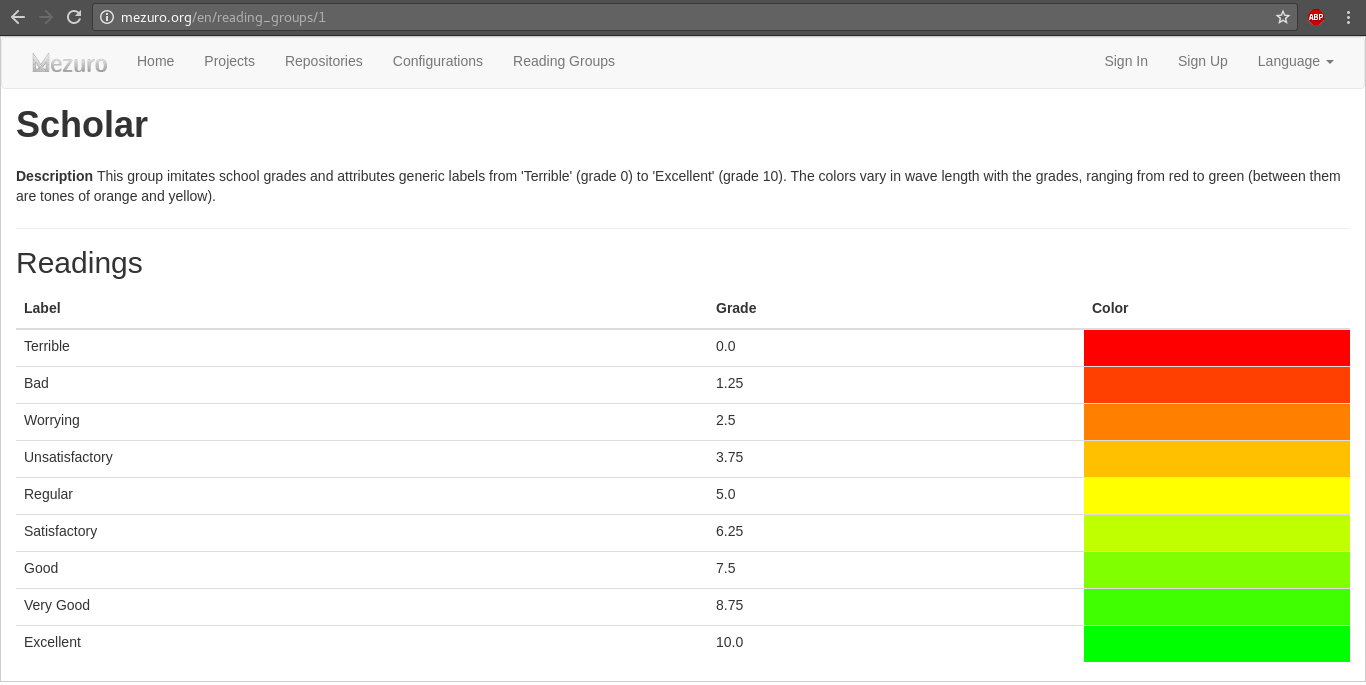
\includegraphics[width=\textwidth]{figures/ReadingGroup.png}
            \label{fig:feature1}
        \end{center}
    \end{figure}
\end{block}

\begin{block}{Next Steps}
    \begin{itemize}
        \item Front-end enhancement
        \item Improvement of processing elapsed time
        \item Auto-detection of repository language
        \item Migrate code management to Gitlab
    \end{itemize}
\end{block}
